\chapter{Motivation de l'étude}
Parce que c'est passionnant. \\

Vous ne trouvez pas? \\

\newpage

		\section{figure, et citation (dans le texte et dans la biblio)}
		\label{le_nom_pour_faire_référence_a_cette endroit}
			\subsubsection*{Des références}
Maintenant, je fais référence à cet endroit dans mon texte (lien cliquable) : \ref{le_nom_pour_faire_référence_a_cette endroit} \\
Les liens directs qu'il peut exister entre la mécanique et le et je cite quelque chose de ma biblio en prime \cite{Dupont2017}.


			\subsubsection*{Un peu de mise en page}
\paragraph*{premier paragraphe}
Pour l'effet de style on rajoute des paragraphe.

\paragraph*{Échelle tissulaire.}
Un autre paragraphe. Bim.
		\newpage
		\section{Une liste}
				Voilà la liste (on peut mettre d'autre points/tirets ect...): 
\begin{itemize}[label = $\square$]
\item le premier truc
\item Le second
\item Le troisième
\item etc...
\end{itemize}

		\newpage
		\section{Objectifs : figure centrée}

	
\begin{figure}[!h]
			\centering
			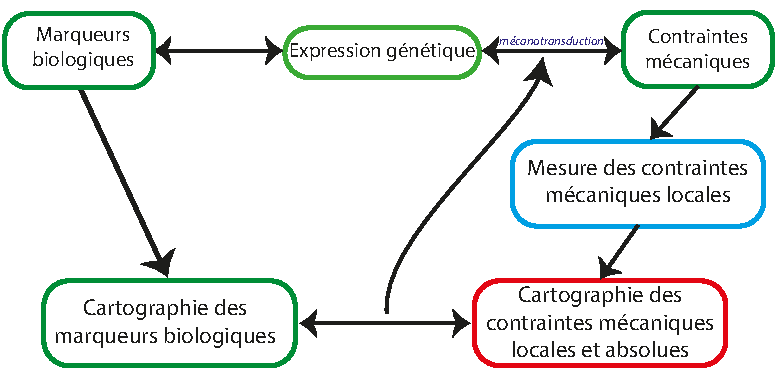
\includegraphics[scale=1]{../1-Introduction/introduction_image/schema_final_objectifs.pdf}
			\caption{la légende}
			\label{fig:schema_objectifs}
			\end{figure}	 		




\chapter{État de l'art}
\label{chap:etat_de_lart}
		\section{Une image en wrap (inclu dans le texte)}	
			\subsection{Définitions}
		\begin{wrapfigure}[14]{i}{8cm}
    		%\centering
   	 		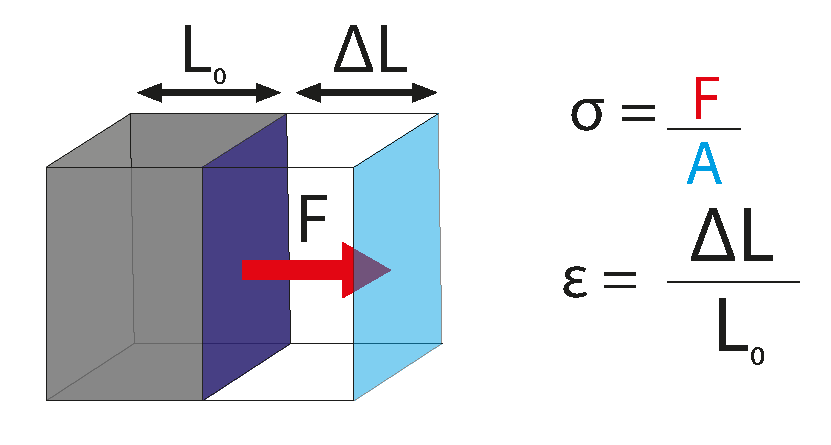
\includegraphics[scale = 0.6]{../1-Introduction/introduction_image/sigma_def_1.pdf}
    		\caption{la légende}
   			\label{fig:le_nom}
\end{wrapfigure}
		
					
				\subsubsection*{Les contraintes}
La suite \\
\chapter{Travail proposé}
Mon troisième chapitre de ma première partie
